\documentclass[12pt, a4paper]{report}
\usepackage{ctex} % 中文的宏包
\usepackage{indentfirst}
\usepackage{graphicx} % 插入圖片的宏包
\usepackage{float} % 設置圖片浮動位置的宏包
\usepackage{subfigure} % 插入多圖時用子圖顯示宏包
\usepackage{listings} % 代碼塊宏包
\usepackage{color} % 代碼高亮
\usepackage[colorlinks,linkcolor=blue]{hyperref} % URL 包
\usepackage[pdf]{graphviz}
\usepackage{tikz}
\usepackage{blindtext}
\usepackage{fancyhdr}
\pagestyle{fancy}

\usetikzlibrary{automata, positioning, arrows}

\definecolor{dkgreen}{rgb}{0,0.6,0}
\definecolor{gray}{rgb}{0.5,0.5,0.5}
\definecolor{mauve}{rgb}{0.58,0,0.82}

\lstset{ %
    %language=Octave,                % the language of the code
    basicstyle=\scriptsize\Hack,           % the size of the fonts that are used for the code
    numbers=none,                   % where to put the line-numbers
    numberstyle=\tiny\color{gray},  % the style that is used for the line-numbers
    stepnumber=2,                   % the step between two line-numbers. If it's 1, each line 
                                    % will be numbered
    numbersep=3pt,                  % how far the line-numbers are from the code
    backgroundcolor=\color{white},      % choose the background color. You must add \usepackage{color}
    showspaces=false,               % show spaces adding particular underscores
    showstringspaces=false,         % underline spaces within strings
    showtabs=false,                 % show tabs within strings adding particular underscores
    frame=single,                   % adds a frame around the code
    rulecolor=\color{black},        % if not set, the frame-color may be changed on line-breaks within not-black text (e.g. commens (green here))
    tabsize=2,                      % sets default tabsize to 2 spaces
    captionpos=b,                   % sets the caption-position to bottom
    breaklines=true,                % sets automatic line breaking
    breakatwhitespace=false,        % sets if automatic breaks should only happen at whitespace
    title=\lstname,                   % show the filename of files included with \lstinputlisting;
                                    % also try caption instead of title
    keywordstyle=\color{blue},          % keyword style
    commentstyle=\color{dkgreen},       % comment style
    stringstyle=\color{mauve},         % string literal style
    escapeinside={\%*}{*},            % if you want to add LaTeX within your code
    morekeywords={*,...}               % if you want to add more keywords to the set
}
\setCJKmainfont{Noto Serif CJK TC} % 主要字體 Noto Serif
\newfontfamily\Hack{Hack} % 代碼字體
\author{軟件 1804 8209180438 黃柏曛}
\date{\today}
\title{TraceTogether 在新冠疫情防控中的应用}
\begin{document}
\maketitle
\lhead{TraceTogether 在新冠疫情防控中的应用}
%\chead{頁首中間的文字}
%\rhead{黃柏曛}

%\lfoot{頁尾左邊的文字}
%\cfoot{第~\thepage~頁}
%\rfoot{頁尾右邊的文字}

\part{摘要}

嚴重特殊傳染性肺炎疫情,是在2019年至2020年間由嚴重急性呼吸系統綜合症冠狀病毒2型(SARS-CoV-2)所引發的全球大流行疫情。疫情擴散對全球航空、旅遊、娛樂、體育、石油市場、金融市場等方面造成巨大影響。 

為了控制疫情,新加坡將開源用來抗疫的 TraceTogether 的 藍芽追蹤 Android APP。

藍芽追蹤技術,實施BlueTrace的應用程序的用戶使用其電話號碼註冊時,後端服務將生成唯一的隨機UserID並將其與用戶的電話號碼相關聯。電話號碼是唯一可個人識別的信息用戶要求。如果發現用戶長時間與感染者接觸,可以使用電話號碼與用戶聯繫。

考慮了藍牙和GPS聯繫人跟踪解決方案。選擇藍牙是因為它能夠以比GPS更低的假陽性率對近距離接觸進行分類。 鑑於GPS精度在室內環境中會下降,因此整個購物中心或摩天大樓都將在單個GPS點的誤差範圍內。 此外,公眾對位置跟踪的警惕和電池消耗的增加可能會阻礙採用。

新加坡接連爆發多起移工(新加坡稱「客工」)宿舍「COVID-19」(2019年新型冠狀病毒疾病)群聚感染。22日,新加坡新增1016起確診病例,當中大多感染者仍是移工,累計病例為1萬141起,總理李顯龍21日發表談話,宣布「阻斷措施」(Circuit Breaker)延長至6月1日。

新加坡被視為善用科技防疫的國家,《海峽時報》報導,李顯龍在談話中說「我們需要每一個人的合作和使用」智慧型手機行動應用程式(App),並鼓勵人們下載TraceTogether。

Smart Nation計劃辦公室計劃的負責人說:“新加坡GovTech現在正在全天候工作,以完成我們的協議參考文件和參考實施,以便其他人可以部署自己的TraceTogether風格-每種都實現BlueTrace協議。” Vivian Balakrishnan在Facebook帖子中說。

“我們相信,將我們的準則發布給全世界將有助於在應對不尊重邊界,政治制度或經濟的全球威脅方面增強信任和協作。”

\tableofcontents

\part{背景}

\begin{figure}[H] % H 為當前位置,!htb 為忽略美學標準,htbp 為浮動圖片
    \centering % 圖片居中
    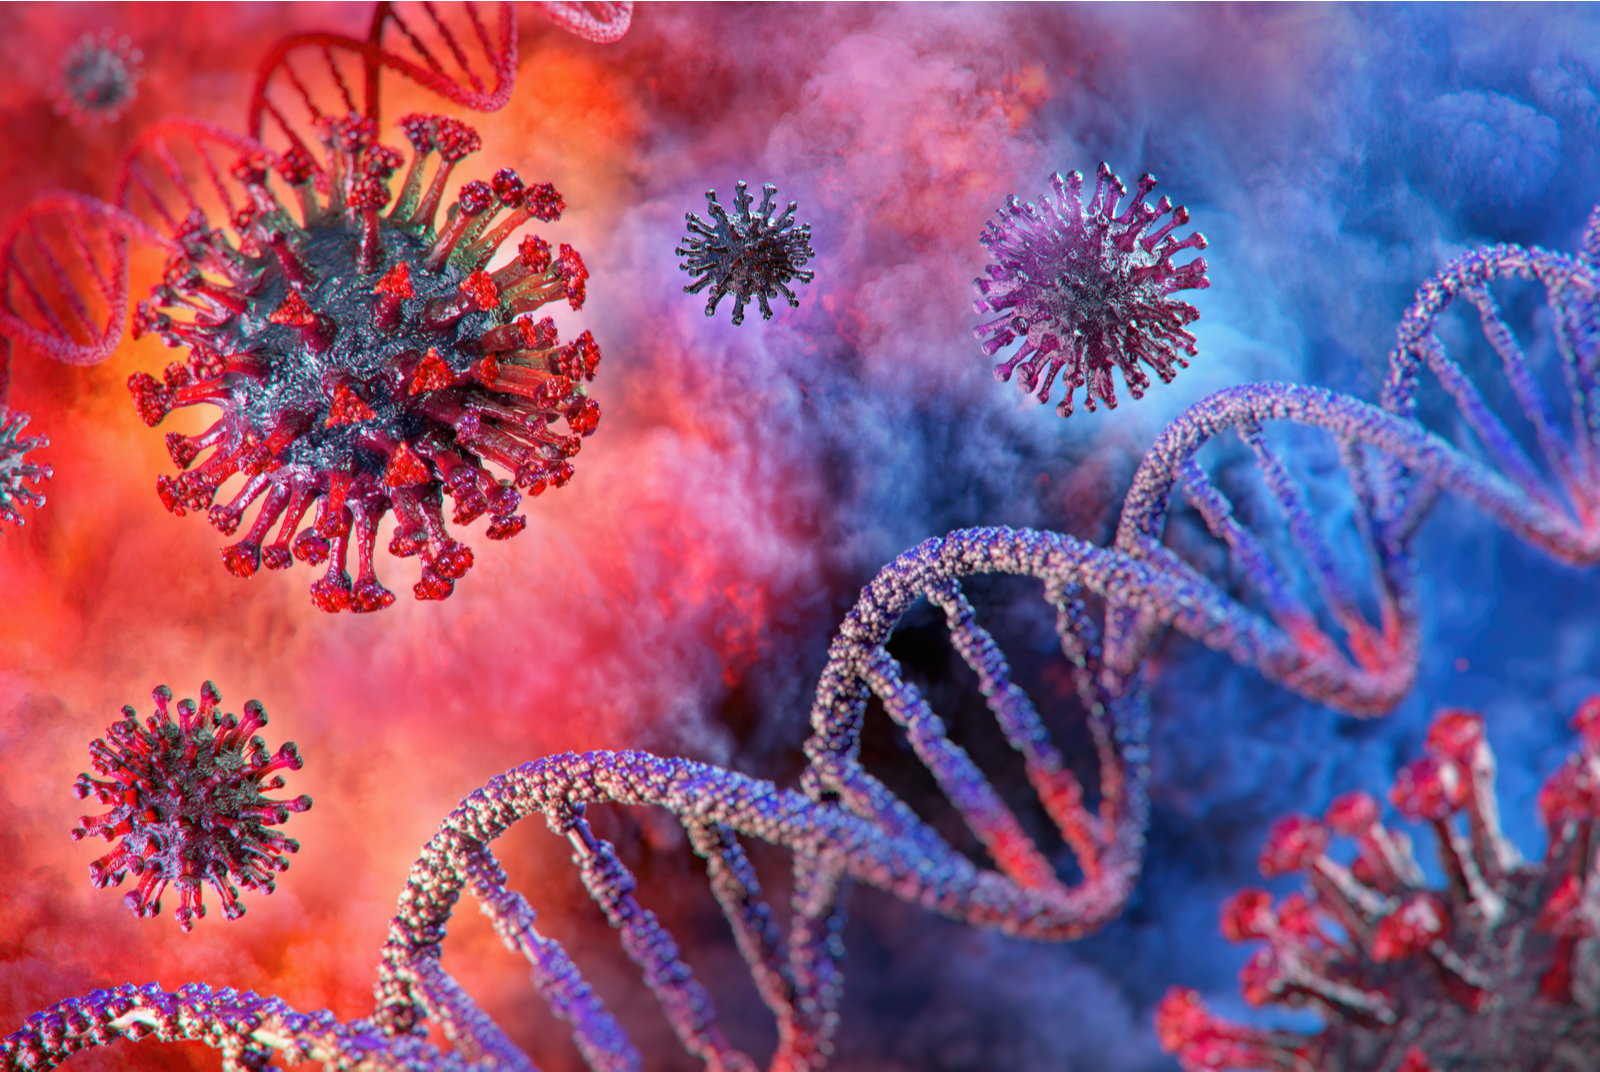
\includegraphics[width=1\textwidth]{background.jpg} % 插入圖片,[] 為圖片大小,{} 是圖片文件
\end{figure}

嚴重特殊傳染性肺炎疫情,是在2019年至2020年間由嚴重急性呼吸系統綜合症冠狀病毒2型(SARS-CoV-2)所引發的全球大流行疫情。疫情在年冬首次爆發於中華人民共和國湖北省武漢市,隨後在2020年初迅速擴散至全球多國,逐漸變成一場全球性大瘟疫,是全球自第二次世界大戰以來面臨的最嚴峻危機。截至2020年4月24日,全球已有220多個國家和地區累計報告超過260萬名確診病例,超過18萬名患者死亡。

目前公認的數據統計認為,首宗感染個案發病時間是2019年12月1日。首位前往醫院就診的患者可能出現於12月12日。12月26日,武漢市呼吸與重症醫學科醫生張繼先最早發現和上報此不明原因肺炎,並懷疑該病屬傳染病。其後該病在武漢市出現大規模疫情。2020年1月23日,武漢市新冠肺炎疫情防控指揮部宣布採取疫區封鎖隔離措施,是近代公共衛生史上第一例將1100萬人口的大城市採取封鎖措施。3月12日,中華人民共和國國家衛生健康委員會宣布,總體上中國大陸本輪疫情流行高峰已經過去。3月23日,中華人民共和國國務院總理兼中央應對疫情小組組長李克強宣布,以武漢市為主戰場的中國本土疫情傳播已基本阻斷,抗疫取得初步成功。

1月13日起,疫情陸續蔓延到泰國、日本及韓國等國家,1月21日波及美國西雅圖,為亞洲以外的首例確診個案。在1月30日中國境外證實有3個國家出現社區傳播,世界衛生組織於當日宣布疫情為「國際公共衛生緊急事件」。2月底義大利、韓國與伊朗三國的確診人數急速增加,29日,世衛組織將疫情的全球風險級別提升為「非常高」。3月11日,世衛組織宣布此次疫情已構成「全球大流行」,世衛組織並於3月13日表示歐洲已經成為當前大流行瘟疫的中心。

病毒潛伏期一般最長多達14天,有個別病例可達24天。即使沒有發燒,沒有感染跡象或僅有輕微感染跡象的感染者也可以將病毒傳染給他人,症狀篩查無法有效檢測。這意味著它比中東呼吸綜合症(MERS)或嚴重急性呼吸系統綜合症(SARS)的疫情更難控制。實際上,這次疫情僅花四分之一的時間就造成SARS事件十倍的確診數字。目前尚無針對新型冠狀病毒的預防疫苗及治療方法。世界衛生組織助理總幹事布魯斯·艾爾沃德認為瑞德西韋是目前「唯一可能具有真正的功效」的藥物;而對症治療則是目前的主要治療方法。全世界目前有至少3種新型冠狀病毒肺炎的預防性疫苗正在處於試驗階段。目前對病症的研究仍存在知識差距,包括病毒來源、病毒發源地、發病機理、病毒的致病性和傳播能力等關鍵因素仍不能確定。

疫情危機持續同時,亦遇上全球醫療用品供應不足的問題。而疫情擴散對全球航空、旅遊、娛樂、體育、石油市場、金融市場等方面造成巨大影響。 

\begin{figure}[H] % H 為當前位置,!htb 為忽略美學標準,htbp 為浮動圖片
    \centering % 圖片居中
    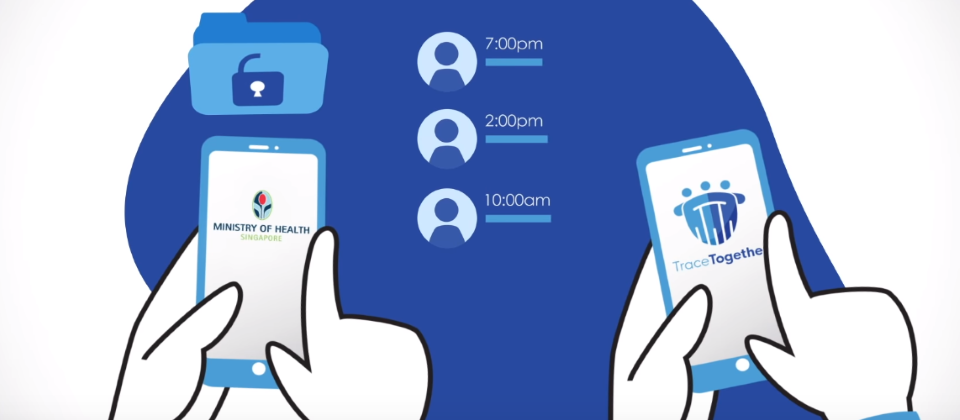
\includegraphics[width=1\textwidth]{tracetogether.png} % 插入圖片,[] 為圖片大小,{} 是圖片文件
\end{figure}

為了控制疫情,新加坡將開源用來抗疫的 TraceTogether Android APP。TraceTogether採用的技術,是由新加坡數位服務部門所研發的藍牙追蹤(BlueTrace)協定,它以藍牙相對訊號強度指標(RSSI),來蒐集與紀錄兩個裝置之間的近距離接觸與時間,相關資訊在手機上的儲存時間為21天。

另一方面,新加坡政府會依據所建立的新型冠狀肺炎確診患者資料庫,追查在過去14天,曾與這些患者近距離接觸的民眾,再提出警告。

為了避免危害使用者的隱私,TraceTogether並不會蒐集手機的位置資訊,且所蒐集的資料只存放在手機上,而且是加密的;除非使用者曾與確診者近距離接觸,否則政府單位永遠不會存取手機上的資料。

此外,在兩支手機互換資訊時,彼此間是以隨機的ID進行通訊,並未涉及任何身分資訊;電話號碼與ID的配對資訊則是存放在另一伺服器上,只有在必要時才會被存取。BlueTrace設備通過在藍牙上交換消息來記錄彼此的遭遇。 為了保護用戶的隱私,這些消息無法透露用戶的身份。 此外,這些消息不能包含靜態標識符,以防止第三方隨時間推移跟踪用戶。

使用BlueTrace的設備既充當中央設備又充當外圍設備,並且可以在這些角色之間交替。當兩個設備連接時,中央設備讀取Pe-ripheral的Encounter Message,然後回寫其自己的Encounter Message。 每個連接都允許在中央和外圍設備之間進行雙向數據交換。 允許雙向通信可以促進對稱性並解決某些設備(可能是可穿戴設備)只能用作外圍設備的局限性。

\part{方法}

\section{藍芽追蹤技術}

\subsection{User registration and assignment of UserID}

\begin{figure}[H] % H 為當前位置,!htb 為忽略美學標準,htbp 為浮動圖片
    \centering % 圖片居中
    \subfigure[User registration]{
    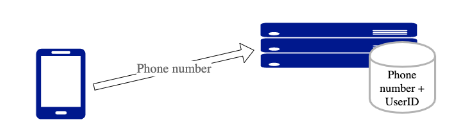
\includegraphics[width=1\textwidth]{userRegister.png}} % 插入圖片,[] 為圖片大小,{} 是圖片文件
\end{figure}

當實施BlueTrace的應用程序的用戶使用其電話號碼註冊時,後端服務將生成唯一的隨機UserID並將其與用戶的電話號碼相關聯。電話號碼是唯一可個人識別的信息用戶要求。如果發現用戶長時間與感染者接觸,可以使用電話號碼與用戶聯繫。用戶註冊不需要電話的BlueTrace替代實現也是可能的。這些可能僅依靠推送通知令牌來提醒單個用戶。

\subsection{Generation of TempIDs}

\begin{figure}[H] % H 為當前位置,!htb 為忽略美學標準,htbp 為浮動圖片
    \centering % 圖片居中
    \subfigure[Format of TempID]{
    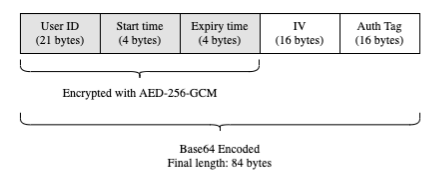
\includegraphics[width=1\textwidth]{foramtOfTempID.png}} % 插入圖片,[] 為圖片大小,{} 是圖片文件
\end{figure}

BlueTrace設備通過在藍牙上交換消息來記錄彼此的遭遇。 為了保護用戶的隱私,這些消息無法透露用戶的身份。 此外,這些消息不能包含靜態標識符,以防止第三方隨時間推移跟踪用戶。 但是,當受感染的用戶將這些消息上載到衛生機構時,該機構必須能夠從消息中獲取聯繫信息。BlueTrace通過讓用戶交換臨時ID(TempID)來解決此問題。 每個TempID包括一個用戶ID,創建的時間和使用AES-256-GCM對稱加密的到期時間,然後使用Base64編碼。 僅健康授權機構擁有用於加密和解密TempID的秘密密鑰。 每個Tem-pID都有一個隨機的初始化矢量(IV)生成.TempID還包括兩個加密參數:IV輸入和一個Auth標籤(用於完整性檢查)。

TempID的壽命很短(15 minutes)。這有助於減少重發機會的機會,從而減輕重犯的影響。 如果惡意用戶通過重新廣播他們的消息來冒充其他用戶,則他們只能在消息出現前的短時間內這樣做。 該持續時間可能低於緊密接觸的閾值持續時間,因此不會導致誤報。

為了即使在互聯網連接不穩定的情況下也能確保設備提供有效的TempID,設備每次都要從衛生機構的後端服務中提取一批轉發的TempID。

BlueTrace設備通過藍牙低功耗(BLE)協議交換消息。在BLE術語中,設備可以使用外設或中央。外設做廣告的服務,以及中樞掃描外圍設備的廣告以連接到其服務。服務是數據的集合,例如特徵,這些數據可以是特定的數據 在設備之間交換,通過中央執行的讀寫操作。 BlueTrace設備在每次“握手”中交換的數據稱為“遇到消息”。

\subsection{BLE handshake flow}

\begin{figure}[H] % H 為當前位置,!htb 為忽略美學標準,htbp 為浮動圖片
    \centering % 圖片居中
    \subfigure[BLE handshake flowD]{
    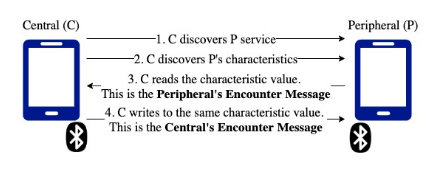
\includegraphics[width=1\textwidth]{BLE_handshake_flow.png}} % 插入圖片,[] 為圖片大小,{} 是圖片文件
\end{figure}

BlueTrace設備通過藍牙低功耗(BLE)協議交換消息。在BLE術語中,設備可以使用外設或中央。外設做廣告的服務,以及中樞掃描外圍設備的廣告以連接到其服務。服務是數據的集合,例如特徵,這些數據可以是特定的數據 在設備之間交換,通過中央執行的讀寫操作。 BlueTrace設備在每次“握手”中交換的數據稱為“遇到消息”。

使用BlueTrace的設備既充當中央設備又充當外圍設備,並且可以在這些角色之間交替。當兩個設備連接時,中央設備讀取Pe-ripheral的Encounter Message,然後回寫其自己的Encounter Message。 每個連接都允許在中央和外圍設備之間進行雙向數據交換。 允許雙向通信可以促進對稱性並解決某些設備(可能是可穿戴設備)只能用作外圍設備的局限性。

\subsection{Scanning and advertising cycles}

BlueTrace設備在可配置週期上進行掃描和通告。 掃描以大約15-20%的佔空比進行,在此期間設備將掃描其他BlueTrace設備作為Central。 設備可以選擇在每個掃描週期的長度和占空比中引入隨機抖動,以避免出現鎖步行為。廣告的佔空比較高,約為90-100%。 建議縮短掃描佔空比,以節省資源。 還建議掃描和廣告工作週期的總和大於1,以確保設備有機會看到彼此。

\section{Bluetooth vs GPS}

考慮了藍牙和GPS聯繫人跟踪解決方案。下表列出了主要區別。選擇藍牙是因為它能夠以比GPS更低的假陽性率對近距離接觸進行分類。 鑑於GPS精度在室內環境中會下降,因此整個購物中心或摩天大樓都將在單個GPS點的誤差範圍內。 此外,公眾對位置跟踪的警惕和電池消耗的增加可能會阻礙採用。

\begin{figure}[H] % H 為當前位置,!htb 為忽略美學標準,htbp 為浮動圖片
    \centering % 圖片居中
    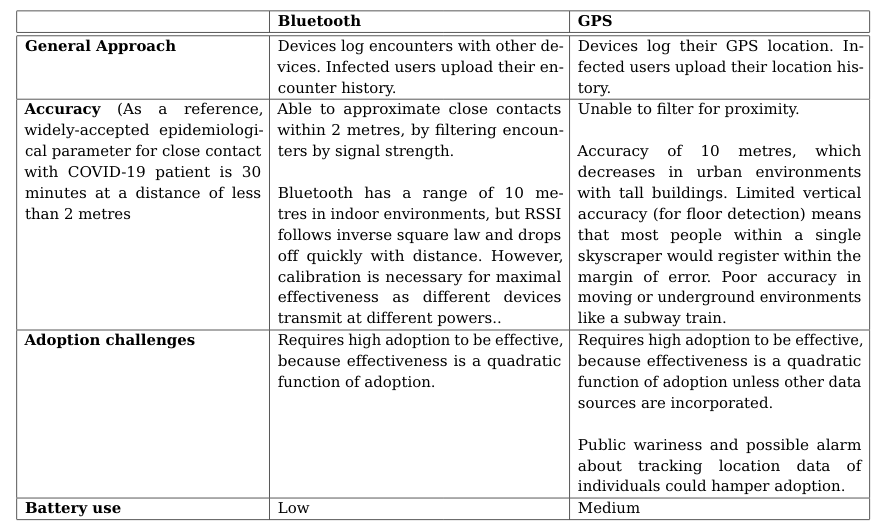
\includegraphics[width=1\textwidth]{blueTooth_VS_GPS.png} % 插入圖片,[] 為圖片大小,{} 是圖片文件
\end{figure}

\subsection{Generation of TempID by backend service vs ondevice}

在參考實現中,TempID是由後端服務以低溫方式生成的。缺點是這需要設備週期性地連接到Internet。我們通過一次發布一批TempID來考慮沒有連接的時間段(另一種方法是將UserID存儲在設備上,並使用非對稱加密密鑰在本地生成TempID,而後端服務則保存相應的解密非對稱加密密鑰可以由後端服務生成,並使用註冊發送給用戶設備,但是,我們發現,這種加密方案使設備的計算需求超出了OS分配的限制,尤其是在後台執行模式下。將設備上的計算需求最小化,服務器端TempID生成具有第二個好處,即允許衛生機構通過記錄每日批TempID的發行記錄來了解應用程序的採用和使用水平及其在流行控制中的潛在有效性。然後可以將其用作公共衛生政策干預措施的參考。 

\subsection{Centralised vs decentralised contact tracing}

BlueTrace設想將分散的鄰近數據收集和日誌記錄結合在一起,並具有集中式的聯繫人跟踪功能;在不使用中央服務器的情況下,將交流消息和遇到的歷史記錄交換並存儲在分散的對等網絡中,我們推遲集中式收集和處理數據診斷到COVID-19的最後時刻,然後在OpenTracereference實現中將此數據提供給受信任的公共衛生機構。根據公共衛生機構所處的現行信任環境,其他轄區可能會有不同的考慮因素,可能會傾向於使用類似的混合模型或完全去中心化的模型。我們看到,純粹的去中心化聯繫追踪系統會帶來各種挑戰。錯誤地聲明自己感染了病毒,將導致其他用戶不必要的焦慮和恐慌,並削弱對系統的信任。因此,為了防止濫用,用戶必須以某種形式的授權將自己標記為積極的COVID-19案例,或者上載遇到的歷史記錄。最終,這必須由具有證書的醫療機構或醫護人員提供,他們可能或可能不是公共衛生當局的傳染病監視系統的一部分,但可能必須通過植根於中央公共衛生當局的信任鏈來獲取上載授權代碼。這也有利於確保將有關這種接觸者追踪系統的流行病以及其有效性和有效性的相關信息提供給公共衛生當局,以幫助規劃公共衛生干預措施。最後,集中化方法的另一個優勢是使人們可以保持在循環評估適當的後續行動。

\part{結果}

新加坡接連爆發多起移工(新加坡稱「客工」)宿舍「COVID-19」(2019年新型冠狀病毒疾病)群聚感染。22日,新加坡新增1016起確診病例,當中大多感染者仍是移工,累計病例為1萬141起,總理李顯龍21日發表談話,宣布「阻斷措施」(Circuit Breaker)延長至6月1日。

新加坡被視為善用科技防疫的國家,《海峽時報》報導,李顯龍在談話中說「我們需要每一個人的合作和使用」智慧型手機行動應用程式(App),並鼓勵人們下載TraceTogether。該App是由政府科技部門研發,透過藍牙訊號進行感染者追蹤(Contact tracing)的工具。

李顯龍指出,該國政府也在開發其他App,「有些關於隱私權的擔憂,但是我們將會權衡,這和讓阻斷措施得以結束帶來的益處,同時維持安全開放。」目前新加坡並未強制每位國民下載。

感染者追蹤,意指追蹤所有曾和感染者接觸的人,進而控制傳染,這是一項極為耗費人力的工作。《紐約時報》報導指出,新加坡1月23日出現了第1例病例後,就開始詳細追蹤了與每一名感染者有過密切接觸的人,也在移工感染病例遽增之前成功掌控疫情。

透過數位裝置的普及,科技可以在追蹤過程中扮演重要角色。TraceTogether是世界第一個藍牙感染者追蹤App,由新加坡政府科技局(GovTech)的政府數碼服務團隊開發,在3月20日推出。

TraceTogether透過藍牙相對訊號強度指標(RSSI)記錄用戶之間的接觸時間,一旦用戶確診,衛生部 (MOH)會根據過去14天的行動繪出地圖。基於數據安全考量,相關紀錄會在手機保留21日,官網中指出「所有數據只會保存在你手機,不會直接分享給衛生部。如果衛生部有需要,他們會尋求你的同意。」

新加坡人口約570萬,《海峽時報》報導,4月1日時,新加坡國家發展部長Lawrence Wong表示,TraceTogether約有100萬下載次數,意即約6人中有1人下載。《路透社》報導,TraceTogether在3月中剛推出時,新加坡確診病例為385例,來到李顯龍發表談話的21日,累計確診已超過9000例,TraceTogether仍然維持大約5人中有1人下載。

\part{結論}

然而在實際使用上 TraceTogether 依然不受大眾信用,我們可以從此 APP 在 Google Play 和 Apple Store 上的評分來看此應用程序依然有許多問題,像是後台耗電、個資隱私問題、還有程序優化。

\begin{figure}[H] % H 為當前位置,!htb 為忽略美學標準,htbp 為浮動圖片
    \centering % 圖片居中
    \subfigure[TraceTogether on Google Play]{
    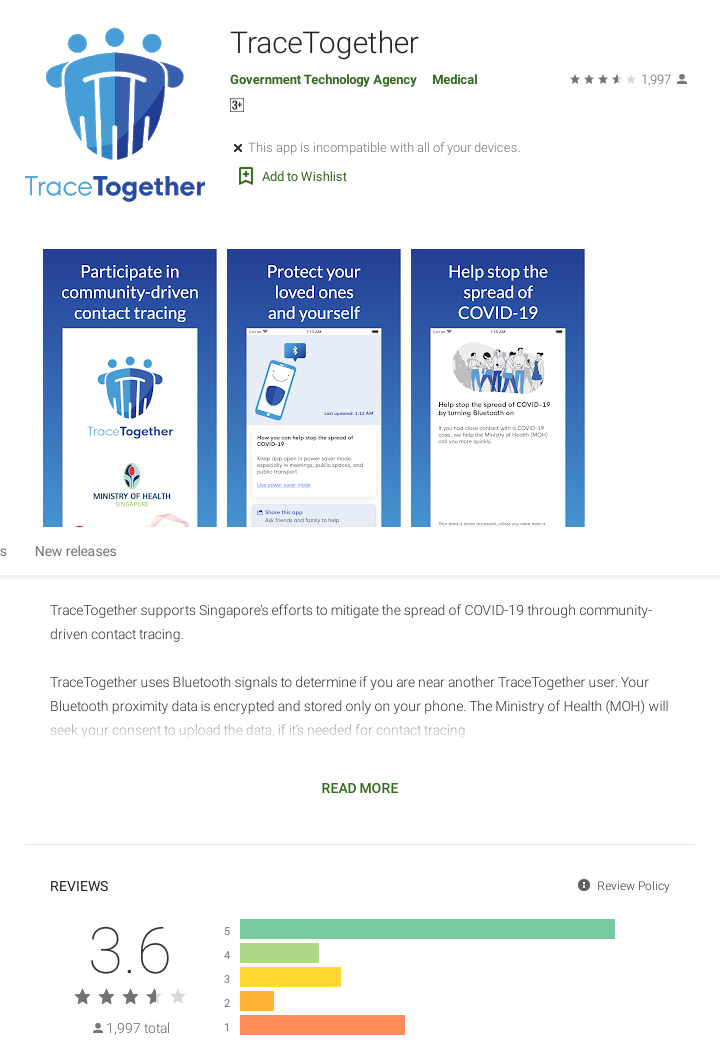
\includegraphics[width=0.4\textwidth]{AppsOnGooglePlay.png}} % 插入圖片,[] 為圖片大小,{} 是圖片文件
    \subfigure[TraceTogether on App Store]{
    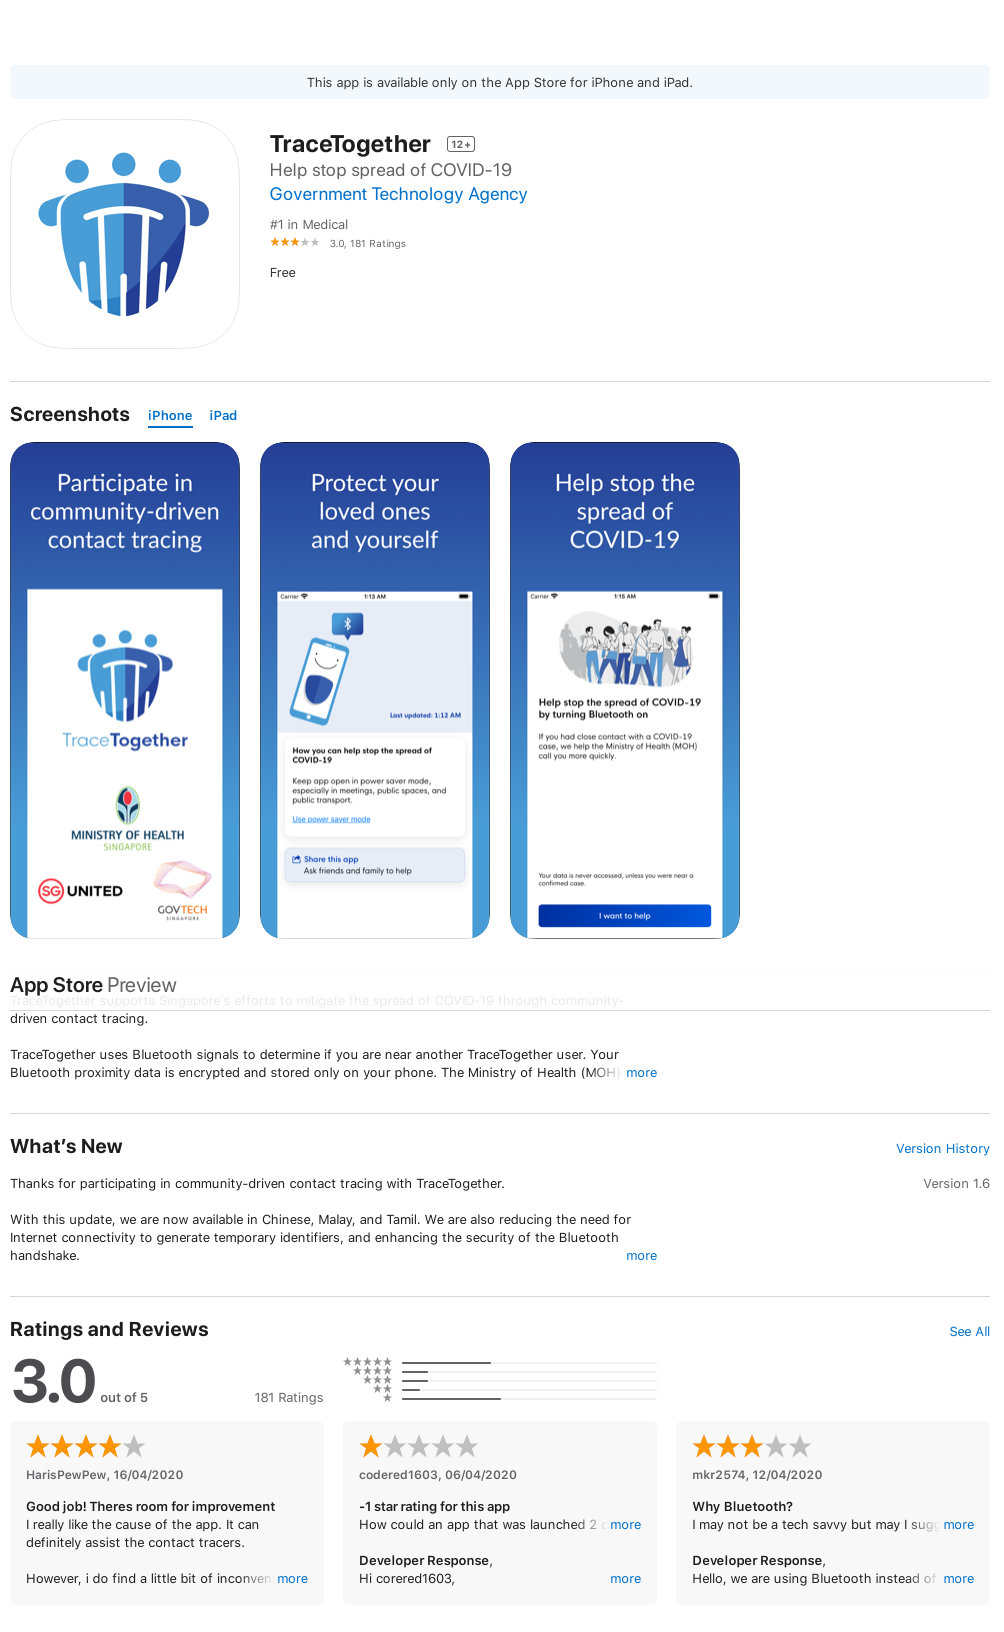
\includegraphics[width=0.4\textwidth]{AppOnAppleStore.png}}
\end{figure}

我們依然能看到即使藍芽追蹤的技術有確保隱私個資的洩漏機制,仍然無法獲取部份人的信任,但是為有效控制疫情全球進最大的努力並使用這類技術避免疫情擴散。

澳大利亞首席醫學官布倫丹·墨菲(Brendan Murphy)表示,該國一直在密切關注新加坡為防止COVID-19進一步傳播所採取的措施,其中包括新加坡已採用的一些技術。

墨菲在新西蘭國會聽證會上說,澳大利亞“非常熱衷”使用新加坡的冠狀病毒接觸追踪應用程序TraceTogether。

他說:“我們實際上已經從新加坡獲得了代碼,我們非常熱衷於使用它,甚至比新加坡更廣泛地使用它。”

“顯然,與社區進行了一次關於其可接受性的對話,但是我們認為,TraceTogether應用程序的構想確實非常出色,如果您對其進行了適當的編程並獲得了正確的社區支持,那麼我們“正在積極地將其視為一項措施的一部分,該措施可能被用於考慮放鬆措施。”

TraceTogether應用程序輕按藍牙信號以檢測附近的其他參與移動設備,從而使它們可以識別需要時保持密切聯繫的那些設備。

該應用程序能夠估計TraceTogether智能手機之間的距離以及此類交互的持續時間。

它可以識別參與的TraceTogether用戶,這些用戶彼此之間相距不超過30米,且相距不超過2米。然後,將數據捕獲,加密並在用戶手機上本地存儲21天,這涵蓋了病毒的潛伏期。

TraceTogether基於BlueTrace協議構建,該協議由新加坡政府技術局的政府數字服務團隊設計。

上個月,新加坡政府宣布將開源該應用程序。

Smart Nation計劃辦公室計劃的負責人說:“新加坡GovTech現在正在全天候工作,以完成我們的協議參考文件和參考實施,以便其他人可以部署自己的TraceTogether風格-每種都實現BlueTrace協議。” Vivian Balakrishnan在Facebook帖子中說。

“我們相信,將我們的準則發布給全世界將有助於在應對不尊重邊界,政治制度或經濟的全球威脅方面增強信任和協作。”

TraceTogether目前擁有超過100萬用戶。

談到取消澳大利亞政府針對COVID-19採取的一些措施時,墨菲說,只有在絕對有信心擁有一個能夠“積極”鎖定的真正良好的公共衛生應對系統的情況下,才可以放鬆管制。爆發。

“我們正在探索用於聯繫追踪的應用程序建議,現在我們在各州和領地擁有數千名公共衛生工作人員……唯一可以放鬆的方法是,如果您有能力真正進入努力控制疫情,”他說。

“如有必要,我們將更加努力。”

墨菲說,目前在澳大利亞要進行三天的聯繫追踪。

影子總檢察長馬克·德雷福斯(Mark Dreyfus)在周三向媒體發表講話時說,要使跟踪應用程序正常工作,需要公眾充分信任並信任公眾,他們的隱私將受到保護。

他說:“只有在公眾廣泛接受的情況下,跟踪應用程序才能工作,因此很大一部分澳大利亞人準備將其安裝在手機上。”

“政府在這一領域的記錄不是很好。他們沒有被證明能夠建立信心,例如,在我的健康記錄,電子保存澳大利亞的健康記錄以及整個危機期間,我不得不說政府事實證明,這種方式並不能很好地吸引澳大利亞人的信任。

“它需要在這個跟踪應用程序上做得更好,因為我再說一遍,除非澳大利亞人信任,有信心,並且將這個應用程序上傳到手機上將保護他們的隱私,否則它將無法正常工作。”

在撰寫本文時,世界衛生組織報告說,已經確認了近180萬例病例,其中有11.7萬多人死於該病毒。澳大利亞報告了約6,400例病例,其中61人死亡。

澳大利亞已進行了336,000多次測試。



\part{Reference}

\begin{itemize}
    \item \href{https://www.tracetogether.gov.sg/}{TraceTogether, safer together}
    \item \href{https://zh.wikipedia.org/wiki/2019%E5%86%A0%E7%8A%B6%E7%97%85%E6%AF%92%E7%97%85%E7%96%AB%E6%83%85}{嚴重特殊傳染性肺炎疫情 - 維基百科}
    \item \href{https://futurecity.cw.com.tw/article/1336}{【科普長文慎入】披羊皮的大野狼!新冠病毒裝無害入侵人體 7種老藥新用抓「詐騙」- 未來城市}
    \item \href{https://www.ithome.com.tw/news/136577}{新加坡將開源用來抗疫的TraceTogether技術}
    \item \href{https://bluetrace.io/static/bluetrace_whitepaper-938063656596c104632def383eb33b3c.pdf}{BlueTrace: A privacy-preserving protocol forcommunity-driven contact tracing across borders}
    \item \href{https://www.thenewslens.com/article/134198}{手機App如何協助追蹤感染者?新加坡總理李顯龍:「我們需要每一個人的合作」}
    \item \href{https://play.google.com/store/apps/details?id=sg.gov.tech.bluetrace&hl=en_US}{TraceTogether on Google Play}
    \item \href{https://apps.apple.com/sg/app/tracetogether/id1498276074}{TraceTogether on App Store}
    \item \href{https://www.zdnet.com/article/australia-looks-to-go-harder-with-use-of-covid-19-contact-tracing-app/}{Australia looks to go harder with use of COVID-19 contact tracing app}
\end{itemize}

\end{document}